\section{Resultados}

\subsection{Cronograma de Atividades}
\frame
{
\frametitle{\emph{Milestones} estabelecidas}
\begin{itemize}
	\item Até Junho/2011:
	\begin{itemize}
		\item Levantamento de requisitos.
		\item Pesquisa sobre o problema.
		\item Pesquisa de metodologia e ferramentas.
		\item Estabelecimento da arquitetura do sistema.
	\end{itemize}
	\item Julho/2011:
	\begin{itemize}
		\item Início da codificação.
		\item Criação dos módulos.
		\item Implementação inicial do \emph{Core} e do \emph{Importer}.
		\item Funcionamento de consultas simples entre \emph{Stops}.
	\end{itemize}
	\item Agosto/2011:
	\begin{itemize}
		\item Suporte a caminhadas entre as \emph{Stops}.
		\item Implementação inicial da Interface \emph{Web}.
		\item Consultas baseadas em latitude e longitude.
	\end{itemize}
\end{itemize}
}
\frame
{
\frametitle{\emph{Milestones} estabelecidas}
\begin{itemize}
	\item Setembro/2011:
	\begin{itemize}
		\item Suporte de \emph{Shapes} no cliente e no \emph{Core}.
		\item Aprimoramento da Interface \emph{Web}.
		\item Consultas com horário de partida.
	\end{itemize}
	\item Outubro/2011:
	\begin{itemize}
		\item Suporte a tarifas.
		\item Início da implementação do cliente Android.
	\end{itemize}
\end{itemize}
}

\subsection{Metodologia Empregada}
\frame
{
\frametitle{Metodologia Empregada}
\begin{figure}
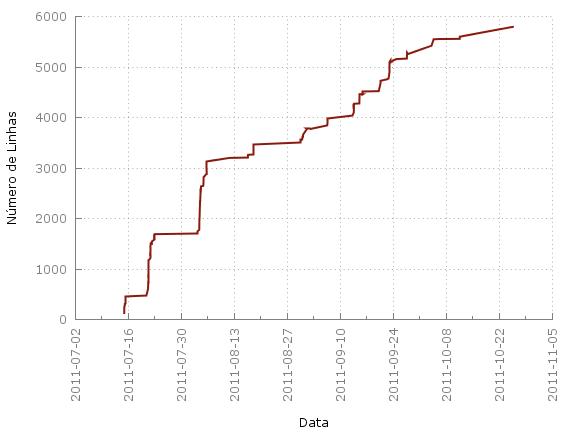
\includegraphics[width=0.7\textwidth]{./imgs/lines_of_code.png}
\caption{Evolução do número de linhas de código do projeto ao longo do desenvolvimento}
\tiny
Fonte: autoria própria.
\end{figure}
}

\frame
{
\frametitle{Metodologia Empregada}
\begin{figure}
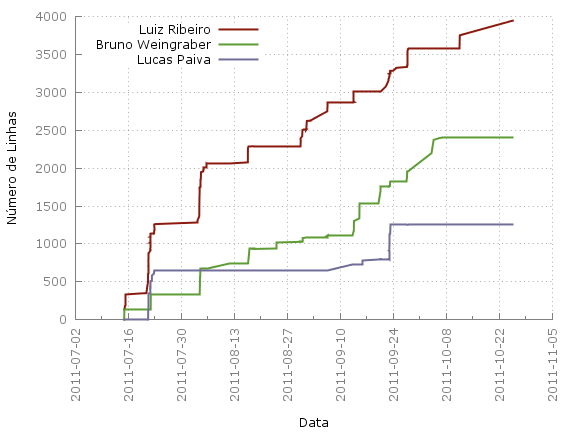
\includegraphics[width=0.7\textwidth]{./imgs/lines_of_code_by_author.png}
\caption{Evolução do número de linhas de código do projeto por programador ao longo do processo de desenvolvimento}
\tiny
Fonte: autoria própria.
\end{figure}
}

\frame
{
\frametitle{Metodologia Empregada}
\begin{figure}
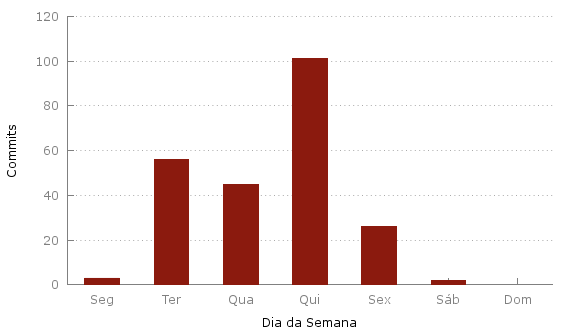
\includegraphics[width=0.7\textwidth]{./imgs/day_of_week.png}
\caption{Número de \emph{commits} por dia de semana}
\tiny
Fonte: autoria própria.
\end{figure}


}

\frame
{
\frametitle{Metodologia Empregada}
\begin{figure}
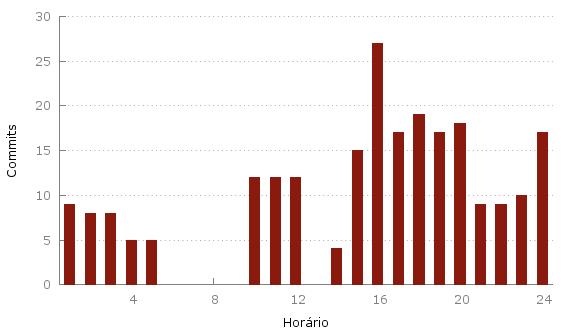
\includegraphics[width=0.7\textwidth]{./imgs/hour_of_day.png}
\caption{Número de \emph{commits} por horário}
\tiny
Fonte: autoria própria.
\end{figure}
}

\subsection{Performance do Sistema}
\frame
{
\frametitle{Teste de \emph{stress}}
\begin{figure}
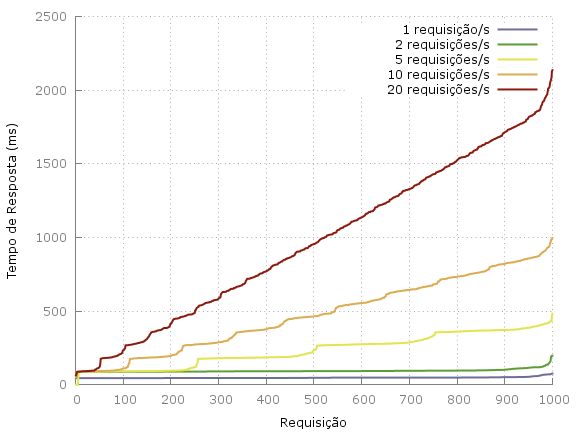
\includegraphics[width=0.7\textwidth]{./imgs/out.png}
\caption{Execução de uma série de consultas simultâneas para avaliação do tempo de resposta do sistema}
\tiny
Fonte: autoria própria.
\end{figure}
}
